\documentclass[a4paper,11pt]{article}
\usepackage[utf8]{inputenc}
\usepackage[T1]{fontenc}
\usepackage[centertags]{amsmath}
\usepackage{amsfonts}
\usepackage{amssymb}
\usepackage{amsthm}
\usepackage{fancyhdr}
\usepackage[left=3cm,top=4cm,right=3cm,bottom=3cm,headheight=3.8cm]{geometry}
\usepackage[singlespacing]{setspace}
\usepackage{natbib}

\fancyhf{}
\pagestyle{fancy}
\usepackage{tikz}
\usetikzlibrary{calc}
\renewcommand{\headrulewidth}{0pt}
\renewcommand{\footrulewidth}{0pt}
\fancyhead[l]{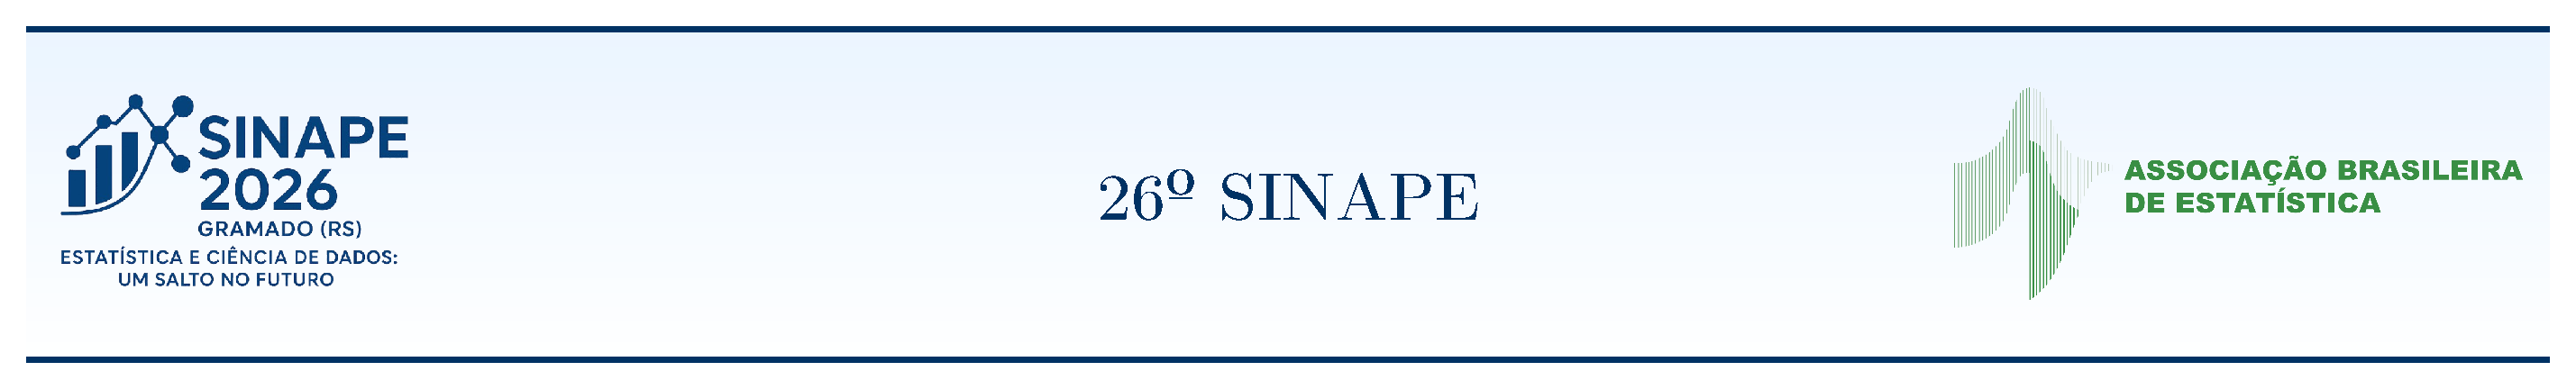
\includegraphics[width=1.1\textwidth]{topo-sinape-2026.pdf}}
\fancyheadoffset{0.05\textwidth}

\setlength{\parindent}{0pt}



\begin{document}


\begin{center}
\Large{\textbf{Inferência causal em dados funcionais via transformadas de ondaletas: do pré-processamento à estimação em tempo real}}
\end{center}

\begin{center}
    Moisés Augusto Farias da Silva
    \footnote[1]{Instituto de Matemática, Estatística e Computação Científica, Universidade Estadual de Campinas - moisesdff8@gmail.com}

    Alex Rodrigo dos Santos Sousa
    \footnote[2]{Instituto de Matemática, Estatística e Computação Científica, Universidade Estadual de Campinas - asousa@unicamp.br}

    \vspace{0.5cm}
    \large{\textbf{Resumo}}
\end{center}

Este trabalho propõe uma metodologia para o problema da inferência causal em dados funcionais, com foco na estimação de efeitos causais médios em trajetórias temporais. Tradicionalmente, a literatura de inferência causal funcional recorre a métodos de suavização globais, como \emph{B-splines}, que impõem suposições estritas de regularidade. Essas restrições dificultam o processamento sequencial de trajetórias e costumam ferir a causalidade operacional, isto é, a direcionalidade rigorosa do tempo. Como alternativa, este trabalho propõe a utilização de transformadas de ondaletas, implementadas através do \emph{lifting scheme}, atuando como uma etapa de pré-processamento. Para além da obtenção de melhores estimativas em um escopo mais amplo de funções, esta dissertação também contribui com a literatura ao viabilizar a estimação do efeito médio de tratamento funcional (\(\mathrm{FATE}\)) em tempo real. Para isso, desenvolvemos o pacote \texttt{rLifting} em linguagem \texttt{R}, com arquitetura unificada em \texttt{C++}, capaz de garantir alta eficiência computacional e fornecer suporte adequado a janelas móveis em atualizações sequenciais. A metodologia foi avaliada via estudos de simulação de Monte Carlo, em que comparamos estimadores baseados em ondaletas (\emph{offline} e \emph{online}) contra abordagens estabelecidas baseadas em \emph{splines}. Os resultados evidenciam que, em cenários caracterizados por descontinuidades e alta irregularidade temporal, as ondaletas superam os métodos clássicos, atingindo menor viés de reconstrução e assegurando coberturas simultâneas nominais através de inferência não paramétrica via \emph{bootstrap}. Ademais, a modalidade \emph{online} apresentou latência computacional na ordem de microssegundos em cada atualização. Concluímos, assim, que a abordagem proposta atua como uma solução analítica rápida, robusta e preservadora da causalidade para a inferência em fluxos contínuos de dados funcionais.

\vspace{0.5cm}
\textbf{Palavras-chave:} Inferência Causal; Dados Funcionais; Ondaletas; \textit{Lifting Scheme}; Tempo Real.

\end{document}
